\chapter{Задание для тренировки}

\textbf{Вариант}: 1

\textbf{Задание}: 

\begin{enumerate}
	\item Дополнить временной план проекта, подготовленный на предыдущем этапе
	(лабораторная работа № 1), информацией о ресурсах и определить стоимость
	проекта.
	\item Для этого заполнить ресурсный лист в программе MS Project, принимая во
	внимание, что к реализации проекта привлекается не более 11 исполнителей.
	\item Предусмотреть, что стандартная ставка ресурса составляет 120 руб./день.
	\item Произвести назначение ресурсов на задачи в соответствии с таблицей. С учетом
	того, что квалификация ресурсов одинаковая, при назначении ресурсов
	использовать процент загрузки.

	\begin{table}[H]
		\begin{center}
			\begin{tabular}{|c|c|}
				\hline
				\bfseries Название работы & \bfseries Количество исполнителей (чел.) \\\hline
				Работа A & 2 \\\hline
				Работа B & 6 \\\hline
				Работа C & 2 \\\hline
				Работа D & 5 \\\hline
				Работа E & 4 \\\hline
				Работа F & 6 \\\hline
				Работа G & 1 \\\hline
				Работа H & 7 \\\hline
				Работа I & 1 \\\hline
				Работа J & 4 \\
				\hline
			\end{tabular}
		\end{center}
	\end{table}

	\item На 3-й день реализации работы В арендуется оборудование по ставке 5 тыс. руб.
	в неделю. На его установку и наладку необходимо выделить 2 тыс. рублей.

\end{enumerate}

\textbf{Результат}:

Были добавлены 11 исполнителей и оборудование для работы B.

\begin{figure}[H]
	\begin{center}
		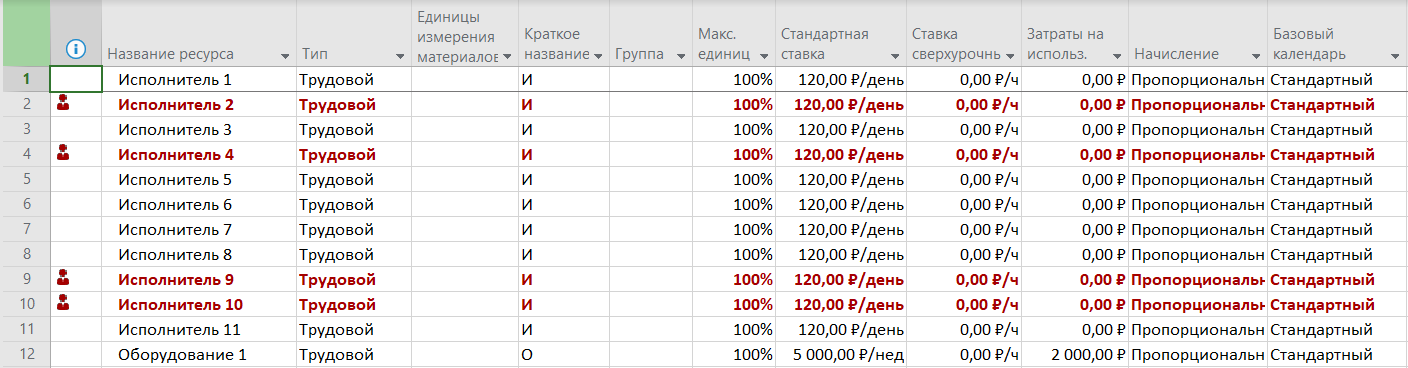
\includegraphics[width=\textwidth]{imgs/task_0_0.png}
	\end{center}
\end{figure}

Была добавлена задержка для оборудования.

\begin{figure}[H]
	\begin{center}
		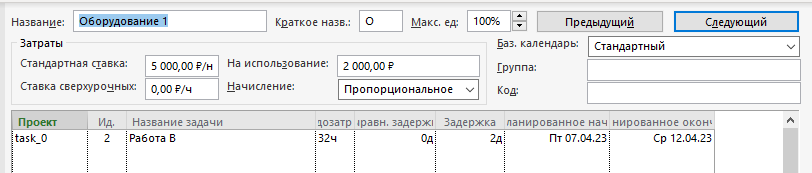
\includegraphics[width=\textwidth]{imgs/task_0_1.png}
	\end{center}
\end{figure}

Результат проделанных действий:

\begin{figure}[H]
	\begin{center}
		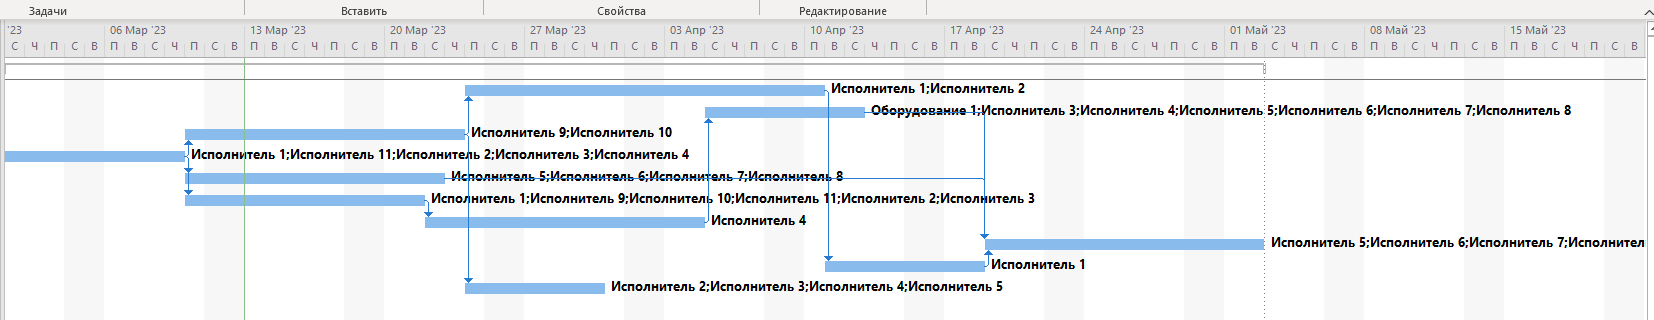
\includegraphics[width=\textwidth]{imgs/task_0_2.png}
	\end{center}
\end{figure}

\begin{figure}[H]
	\begin{center}
		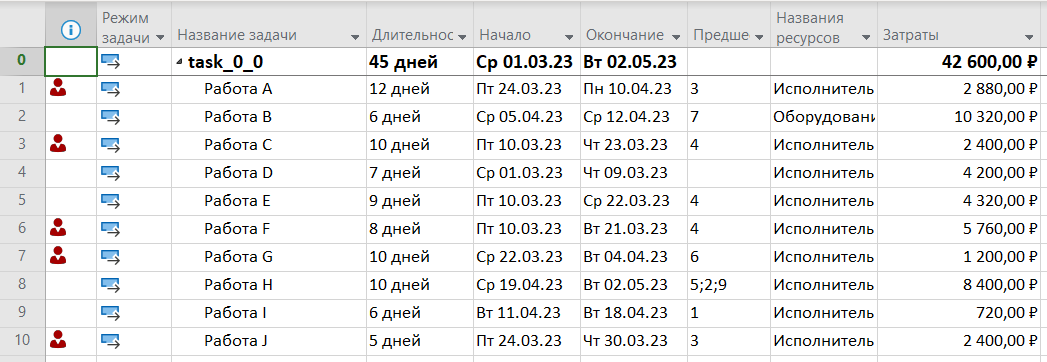
\includegraphics[width=\textwidth]{imgs/task_0_3.png}
	\end{center}
\end{figure}

Видно, что исполнители 2, 4, 9 и 10 перегружены и в их расписании есть наложения задач.

\begin{figure}[H]
	\begin{center}
		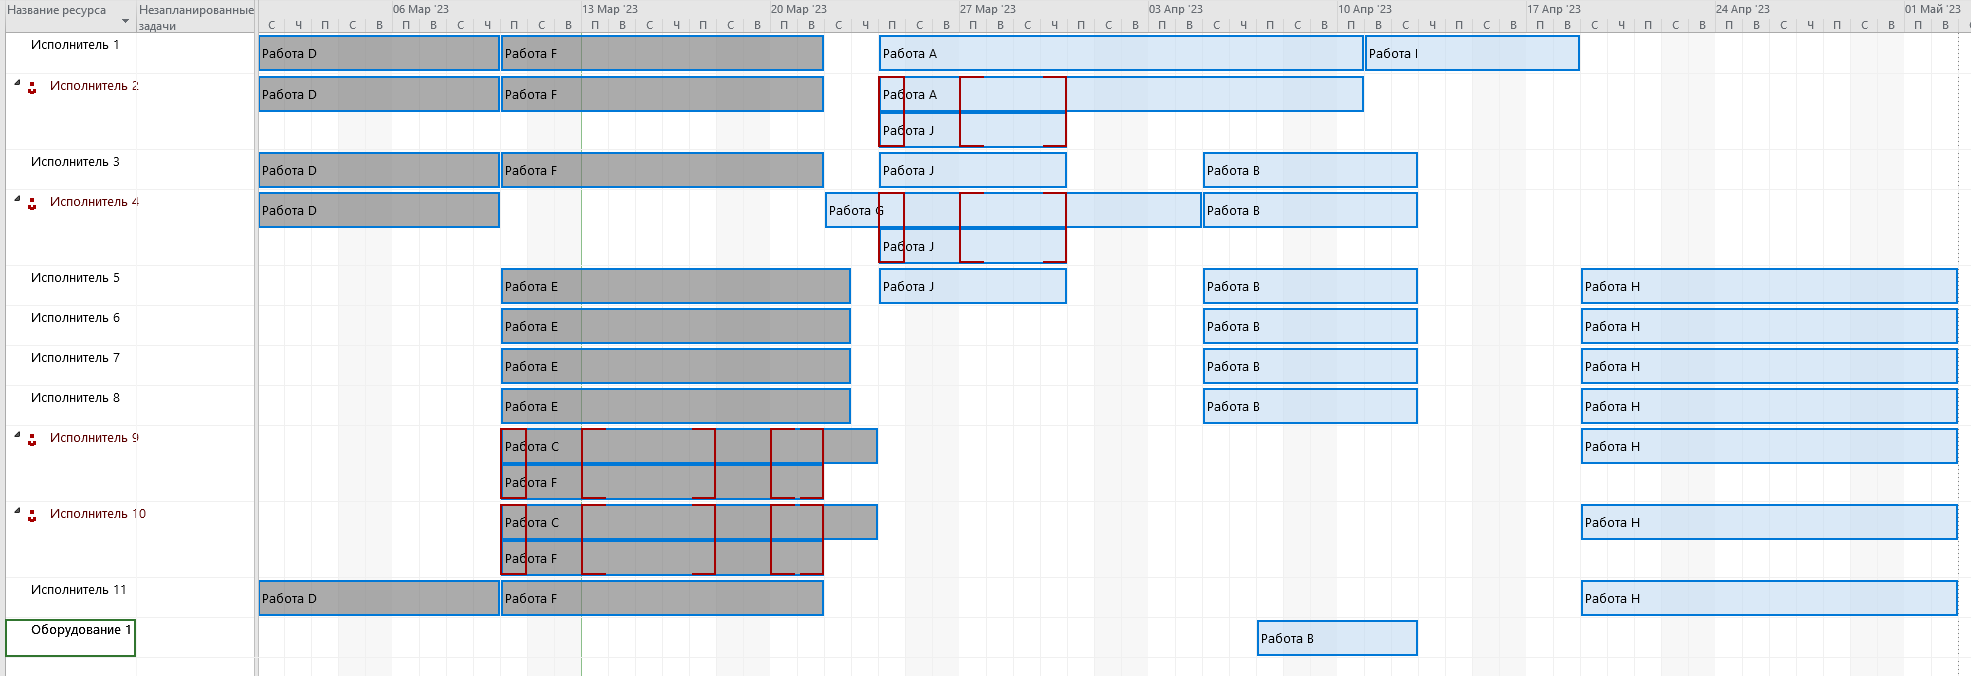
\includegraphics[width=\textwidth]{imgs/task_0_4.png}
	\end{center}
\end{figure}